\documentclass[aspectratio=169, 9pt]{beamer}

%%%%%%%%%%%%%%%%%%%%%%%%%%%%%%%%%%%%%%%%%%%%%%%%%%%%%%%%%%%%%%%%%%%%%%%%%%%%%%%%%%%
%   This template is modified by Mirza Akbar Ali (CUI). All rights to the original template are reserved to the owner and I acknowledge all their contributions towards the advancement of efficient presentation styles using LaTeX and Beamer.  Furthermore, anyone who want to use this template is allowed to make best out of this template and go for the best presentation of their project. Good Luck 


%%%%%%%%%%%%%%%%%%%%%%%%%%%%%%%%%%%%%%%%%%%%%%%%%%%%%%%%%%%%%%%%%%%%%%%%%%%%%%%%%%
%   Do not delete any of the following package, how ever you can include more packages as per you requirements.
\usetheme{Warsaw}
\usepackage[style=verbose]{biblatex}
\usepackage{filecontents}
\addbibresource{bibliography.bib}
\usepackage{tikz}
\usepackage{times}
\usepackage{hyperref}
\usepackage{graphicx} % Allows including images
\usepackage{booktabs} % Allows the use of \toprule, \midrule and \bottomrule in tables
\usepackage{amsmath}
\usepackage{amsfonts}
\usepackage{amssymb}
\usepackage{subcaption}
\usepackage{siunitx} 
\addtobeamertemplate{block begin}{}{\justifying}
\setbeamertemplate{section in toc}[sections numbered]  % to create content list
\setbeamertemplate{caption}[numbered] % to number the captions
\setbeamerfont{caption}{size=\tiny} % Changes the font size of the captions
\setbeamerfont{footnote}{size=\tiny} % Changes the font size of footnotes
\setbeamerfont{footnotemark}{size=\miniscule}
\setbeamertemplate{footline}{%
  \leavevmode%
  \hbox{\begin{beamercolorbox}[wd=.5\paperwidth,ht=4.5ex,dp=2.125ex,leftskip=.3cm plus1fill,rightskip=.3cm]{author in head/foot}%
    \usebeamerfont{author in head/foot}\insertshortauthor
  \end{beamercolorbox}%
  \begin{beamercolorbox}[wd=.5\paperwidth,ht=4.5ex,dp=2.125ex,leftskip=.3cm,rightskip=.3cm plus1fil]{title in head/foot}%
    \usebeamerfont{title in head/foot}
    \parbox{.45\paperwidth}{\inserttitle\hfill \insertframenumber\,/\,\inserttotalframenumber}
  \end{beamercolorbox}}%
  \vskip0pt%
}

%%%%%%%%%%%%%%%%%%%%%%%%%%%%%%%%%%%%%%%%%%%%%%%%%%%%%%%%%%%%%%%%%%%%%%%%%%%%%%%%%%%%%
%%%%%%%%%%%%%%%%%%%%%%%%%%%%%%%%%%%%%%%%%%%%%%%%%%%%%%%%%%%%%%%%%%%%%%%%%%%%%%%%%%%%%
%       Add You Name, Registration Number, Presentation Title, Supervisor Name

\author[Name \quad \quad Registration Number ]{Name \\ Registration Number}
\title{Presentation Title}
\subtitle{Synopsis/Presentation1} % if you do not want this, you can comment this line
\institute[CUI] % (optional)
{
    {\small Supervisor} \\ \vspace{0.5mm} {\normalsize Supervisor Name} \vspace{5mm}
}

%%%%%%%%%%%%%%%%%%%%%%%%%%%%%%%%%%%%%%%%%%%%%%%%%%%%%%%%%%%%%%%%%%%%%%%%%%%%%%%%%%%
%   Main Document Starts Below

\begin{document}

%   Title Slide

\begin{frame}[plain]
    \begin{center}
            \begin{minipage}[c]{0.2\linewidth}
                    \begin{center}
                    
\includegraphics[width=1.3cm, height=1.3cm]{./Graphics/CUI-Logo.png} 
                    \end{center}
            \end{minipage}
            \begin{minipage}[c]{0.5\linewidth}
                    \begin{center}
                    \begin{large}
                    COMSATS University Islamabad \\ \vspace{1mm}Department of Physics
                    \end{large} 
                    \end{center}
            \end{minipage}
    \end{center}
\titlepage 
\end{frame}

%%%%%%%%%%%%%%%%%%%%%%%%%%%%%%%%%%%%%%%%%%%%%%%%%%%%%%%%%%%%%%%%%%%%%%%%%%
% Do not make changes to following begingroup code This creates Table of Content Slide

\begingroup 
    \setbeamertemplate{headline}{}
    \addtobeamertemplate{frametitle}{\vspace*{-\headheight}}{}
    \begin{frame}{Contents}
        \tableofcontents{}
    \end{frame}
\endgroup

%%%%%%%%%%%%%%%%%%%%%%%%%%%%%%%%%%%%%%%%%%%%%%%%%%%%%%%%%%%%%%%%%%%%%%
% You Main Presentation Starts Here


\section{Section 1}

\subsection{Section 1 Subsection 1: Itemizing Part 1}

\begin{frame}{Section 1 Subsection 1: Itemizing Part 1}
    \begin{itemize}
     \setlength{\itemsep}{10pt}
        \item Item 1
        \begin{itemize}
            \item Item 1 Subitem 1
            \item Item 1 Subitem 2
            \item Item 1 Subitem 3
        \end{itemize}
        \item Item 2
        \begin{itemize}
            \item Subitem 1
            \begin{itemize}
                \item Subsubitem 1
            \end{itemize}
            \item Subitem 2
            \begin{itemize}
                \item This is marked subitem \\
                This is unmarked subitem
            \end{itemize}
        \end{itemize}
    \end{itemize}
\end{frame}


\subsection{Section 1 Subsection 2: Itemizing Part 2}

\begin{frame}{Section 2 Subsection 2: Itemizing Part 2}
\begin{itemize}
    \item[Step 1] This is step 1
    \item[Step 2] This is step 2
    \item[Step 3] Yuo can add small equation in text $y=mx+c$ or $x^{3}=2y$
    \item[Step 4] You can add a separate equation
        \begin{align*}
        |\Psi \rangle = \sum_{i} u_{i} | \varphi_{i} \rangle 
    \end{align*}
\end{itemize}
\end{frame}


\subsection{Section 1 Subsection 3: Footnote Citing}

\begin{frame}{Section 1 Subsection 3: Footnote Citing}
\begin{itemize}
    \item This is simple text
    \item This text is footnote cited \footnotemark
    \item Add you resources in bibliography file 
\end{itemize}
        \footnotetext{\cite{AmorphousGraphene}}
\end{frame}


\section{Section 2}

\subsection{Section 2 Subsection 2: Equation}

\begin{frame}{Section 2 Subsection 2: Equation}
    \begin{flushleft}
    \textbf{Name of Some Theorem}
    \end{flushleft} 
    \begin{align}
         \Psi (\Vec{r}+ \Vec{R}) = e^{i\Vec{k}\cdot\Vec{R}}\Psi(\Vec{r})
    \end{align}
    Where
    \begin{itemize}
        \item $\Vec{R}$ is somethin
        \item $\Vec{k}$ is something
    \end{itemize}
\end{frame}


\subsection{Section 2 Subsection 3: Multiple Equations}

\begin{frame}{Section 2 Subsection 3: Multiple Equations}
    \begin{align}
        |\Psi \rangle = \frac{1}{\sqrt{N}} \sum_{i}^{N} e^{i\Vec{k}\cdot\Vec{R}_{i}}|s_{i}\rangle \label{Wavefunc} \\ 
        \frac{1}{\sqrt{N}} \sum_{j=1}^{N} \left[ H_{ij}e^{i\Vec{k}\cdot\Vec{R}_{j}}-\varepsilon e^{i\Vec{k}\cdot\Vec{R}_{i}}\right] = 0 \label{Eq0003}
    \end{align}
    As you can see in equation \ref{Eq0003}. Chcek how i referred to this equation in code. 
\end{frame}


\section{Add Picture or Figure}

\begin{frame}{Add Picture or Figure}
        \begin{minipage}[t]{\linewidth}
            \begin{center}
            \begin{figure}
                \centering
                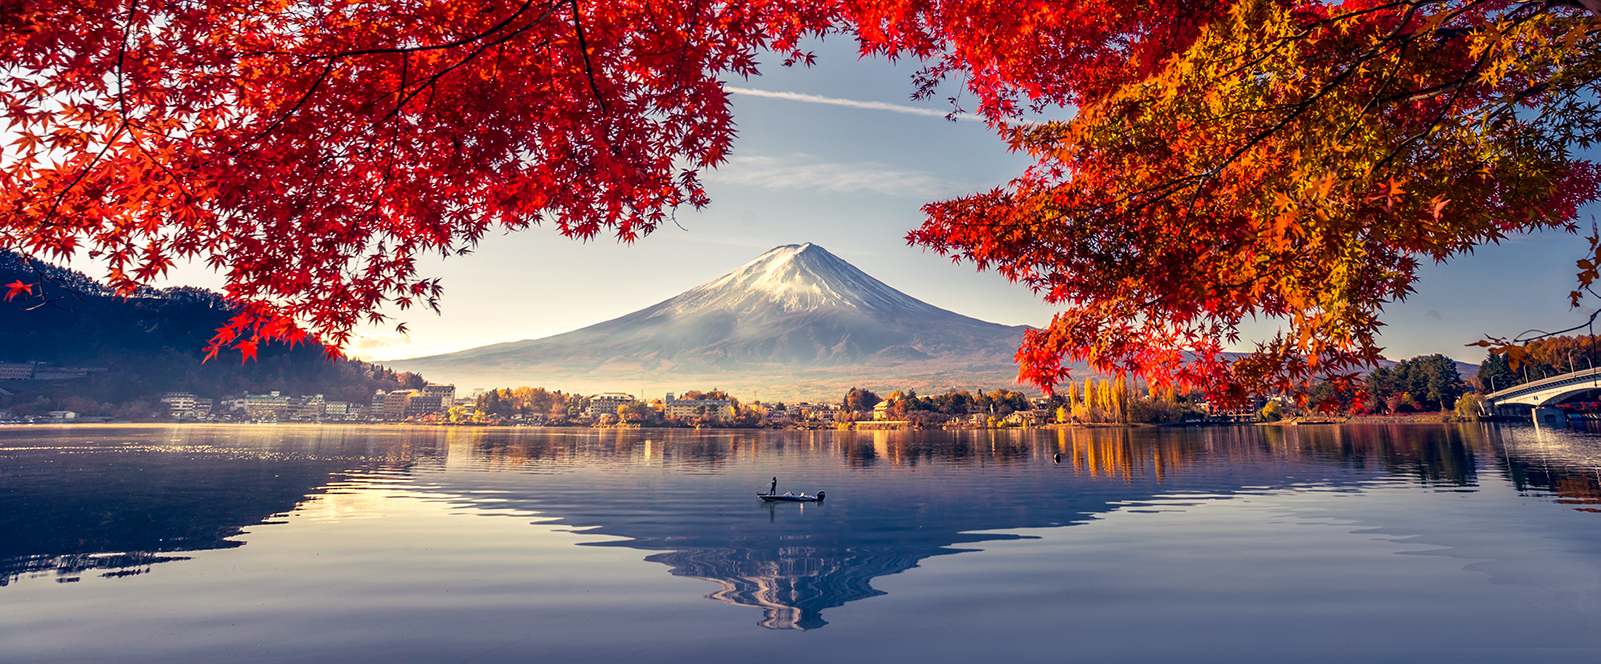
\includegraphics[width=0.7\linewidth]{./Graphics/BeautifulPicture.jpg}
             \caption{This is How you add a beautiful picture}
                \label{BFigure1} %You can use this to refer to this pic
            \end{figure}
            \end{center}
        \end{minipage}
        See the code to check how i referred to this Figure \ref{BFigure1} and upload all your pictures in Graphics folder to create no messy main folder.
\end{frame}

% If you want a references slide at the end of presentation then un comment the following code
%\section*{References}
%\begin{frame}{References}
%\bibliographystyle{IEEEtranN}
%\bibliography{bibliography.bib}
%\end{frame}
\end{document}